\documentclass[]{article}
%Font encoding for swedish
\usepackage[utf8]{inputenc}
\usepackage[T1]{fontenc}

\usepackage{tikz}
\usetikzlibrary{shapes,arrows,calc}


% Title Page
\title{Teknisk rapport\\Grafisk räknare}
\author{}


\begin{document}
\maketitle

\begin{abstract}
\end{abstract}
\section{Inledning}

\section{Apparaten}
Börja gärna med en bild på bygget och redgör för hur apparaten används. Detta blir en kombinerad presentation av konstruktionen och användarhandledning. 
\section{Teori}
Här kan ett videoprojekt beskriva videoformatet, ett MIDI-projekt redogöra för MIDI-standarden ...
\subsection{Reverse polish}
\section{Hårdvaran}
Börja med ett översiktligt blockschema, gå vidare till mera detaljerade blockschemor. Vill man rita figurer och blockschemor på datorn så är Inkscape ett bra alternativ. Handritade figurer och blockschemor är acceptabelt, bara de är snygga och väl läsbara, MEN dessa ska då vara inscannade, dvs avfotograferade figurer och blockschemor är INTE godtagbart.
Beskriv sedan hur de olika blocken fungerar. Tänk på läsbarheten och växla mellan figurer och text. Den här typen av text är ganska "grafisk", då nästan varje mening syftar in i en figur. Var därför noga med att text och figurer stämmer överens.
\subsection{Översikt}

\tikzstyle{block} = [draw, fill=blue!20, rectangle, 
minimum height=3em, minimum width=6em]
\tikzstyle{sum} = [draw, fill=blue!20, circle, node distance=1cm]
\tikzstyle{input} = [coordinate]
\tikzstyle{output} = [coordinate]
\tikzstyle{pinstyle} = [pin edge={to-,thin,black}]

\begin{figure}[h!]
	\centering
	\begin{tikzpicture}[auto, node distance=2cm,>=latex']
	
	
	
	\node [block, node distance=3cm] (cpu) {CPU};
	\node [block, below of=cpu, node distance=2cm] (memory) {Bildminne};
	\node [output, right of=cpu] (foo) {};
	
	
	\draw [<->] (cpu) -- node[near start]{} (memory);
	\node [block, above of=cpu] (keyboarddriver) {Tangentbordsmotor};
	\node [block, node distance=3.5cm, left of=keyboarddriver] (keyboard) {Tangentbord};
	
	\draw [<->] (keyboarddriver) -- node {} (cpu);
	\draw [->] (keyboard) -- node {} (keyboarddriver);
	
	\node [block, node distance=2cm, below of=memory] (driver) {VGA-motor};
	\node [block, right of=driver, node distance=3.5cm] (vga) {Skärm};
	\draw [->] (memory) -- node {} (driver);
	\draw [->] (driver) -- node {} (vga);
	\draw[thick,dotted] ($(keyboarddriver.north west)+(-0.3,0.3)$)  rectangle ($(driver.south east)+(1,-0.3)$) node[pos=0] {FPGA};
	\end{tikzpicture}
	\caption{Översiktligt blockschema.}
\end{figure}

\subsection{CPU}

CPU:n är baserad på icke-pipelinade Björn Lindskogs-datorn. Huvudminnet, och de allra flesta register inklusive de generella, är 32 bitar långa.

\subsubsection{mPC}

Microprogramräknaren. Microninstruktioner har fyra bitar att modifiera räknaren med, vilket sker på positiv klockflank. Koderna gör som följer:
\\

\begin{tabular}{llc}
\textbf{Kod} & \textbf{Funktion} \\
\hline
\texttt{0001} & mPC := ADR \\
\texttt{0010} & mPC := K2(<Given mod>) \\
\texttt{0011} & mPC := K1(<Given Instruktion>) \\
\texttt{1000} & mPC := ADR if flag\_X == \texttt{1} else mPC++ \\
\texttt{1001} & mPC := ADR if flag\_N == \texttt{1} else mPC++ \\
\texttt{1010} & mPC := ADR if flag\_Z == \texttt{1} else mPC++ \\
\texttt{1011} & mPC := ADR if flag\_C == \texttt{1} else mPC++ \\
\texttt{1100} & mPC := ADR if flag\_V == \texttt{1} else mPC++ \\
\texttt{Others} & mPC++
\end{tabular}
\\

\noindent
K2 och K1 är minnen som binder en given mods eller instruktions binärrepresentation till raden i microminnet som har hand om dess del i hämtfasen respektive exekveringsfasen.

\subsubsection{IR}

Instruktionsregistret, 32 bitar, håller i en kopia av instruktionen från huvudminnet som körs för tillfället. Den kan vidare delas upp i OP, GRx, MM, och IR\_ADR som är den instrukionens instruktionskod, GRx-argument, valt mod, samt address-argument.

Man kan i microkoden skriva och läsa till och från IR genom att ange busskoden \texttt{0001} i från-buss respektive till-bus fältet. Att skriva till IR påverkar inte huvudminnet, och därmed inte den egentliga programkoden.

\subsubsection{PC}

Programräknaren, håller koll på instruktion i p\_mem som ska exkaveras. Registret är 22 bitar långt, då detta är fullt tillräckligt för alla rimligt stora program, samt att addressfältet hos en instruktion inte har plats för större tal på sin addressdel: de sista 22 bitarna.

PCsig, bit nummer 18 i microinstruktionen, kan påverka PC. Ett värde på 0 håller PC oförändrad, medan ett värde på 1 inkrementerar den.

PC kan skrivas till via bussen. En från-buss-signal på \texttt{0011} skriver de 22 lägsta bitarna av DATA\_BUS till PC. Den kan även läsas ifrån genom att ange samma busskod på till-buss delen i microminnet.

\subsubsection{ASR}

Addressregistret används i microprocessorn för att peka ut addressen till raden som ska passera som argument. Detta sätts i hämtfasen och beror på vilket mod den dåvarande instruktionen körs med.

Liksom PC är registret av samma anledning 22 bitar långt.

ASR kan läses från och skrivas till via busskoden \texttt{0100}.

\subsubsection{GRx}

De åtta generella registrena: GR0 till och med GR7.

Dessa register är 32 bitar långa och används för att främst hålla i temporära värden åt användaren.

Vektorn g\_reg håller i de åtta registren, och ett av de väljs genom signalen GRx. Denna är bitar 26 till och med 24 hos programinstruktionen som körs för tillfället.

Att skriva eller läsa till det valda generella registret görs via busskuden \texttt{1000}. Det är den som valts i GRx som då interageras med. 

\subsubsection{p\_mem}

Vårt programminne, 32 bitar långt. Då programminne och dataminne är samma minne så syftas här på det delade minnet. Genom att skriva eller läsa härifrån via busskoden \texttt{0010} så kan huvudminnet läsas eller modifieras. Raden i minnet som opereras på utpekas ASR, som sätts automatiskt i hämtfasen.

Det är värt att notera att programminnet initialt sätts till konstanten p\_mem\_c, där då programkod skrivs in.

\subsubsection{save\_at\_p/save\_at\_b/data\_out\_picmem/data\_out\_bitmap}

Signaler för att skriva till bild och bitmapminne. Via busskoden \texttt{0111} skickas de sista 8 bitarna i \texttt{DATA\_BUS} via \texttt{data\_out\_picmem} och \texttt{ASR} till \texttt{save\_at\_p}. Via busskoden \texttt{0110} skickas den sista biten i \texttt{DATA\_BUS} via \texttt{data\_out\_bitmap} och \texttt{ASR} till \texttt{save\_at\_b}. Samtidigt aktiveras en (aktivt hög) write-enable-signal, \texttt{web} vid skrivning till bitmapminnet och \texttt{wep} vid skrivning till bildminnet. Dessa nollställs inte, utan används bara för att undvika odefinierade signaler innan första skrivningen.

\subsubsection{AR/ALU}

I processen titulerad AR finns koden som utgör enhetens ALU.

Här modifieras ackumulatorregistret, AR, (32 bitar), och de fem flaggorna. En rad olika operationer kan utföras på positiv klockflank beroende på koden hos ALU-signalen; de fem första bitarna i mikrominnesinstruktionen som för tillfället körs.

Vid matematiska operationer tolkas AR och bussens värde som ett signerat tvåkomplementstal.

AR:s värde kan senare läggas på bussen genom att ange koden \texttt{0101} i mikrokoden. Den kan dock ej skrivas till direkt.

Nedan följer en tabell över alla ALU-operationer: deras koder, funktion, och modifierade flaggor.
\\

\begin{tabular}{llc}
\textbf{Kod} & \textbf{Funktion} & \textbf{Flaggor påverkade}\\
\hline
\texttt{00000} & \texttt{<Ingenting>} & \\
\texttt{00001} & AR := BUS &  \\
\texttt{00010} & AR := BUS' & \\
\texttt{00011} & AR := 0 & \\
\texttt{00100} & AR := AR+BUS & \texttt{X C V N Z}\\
\texttt{00101} & AR := AR-BUS & \texttt{X C V N Z} \\
\texttt{00110} & AR := AR \textsc{and} BUS & \texttt{{ } C V N Z}\\
\texttt{00111} & AR := \textit{signed\_to\_real}(AR) & \\
\texttt{01000} & AR := \textit{real\_to\_signed}(AR) & \\
\texttt{01001} & AR := AR \textsc{asr} BUS & \texttt{X C V N Z}\\
\texttt{01010} & AR := AR \textsc{asl} BUS & \texttt{X C V N Z}\\
\texttt{01011} & AR := AR+BUS (fixed point) & \texttt{X C V N Z} \\
\texttt{01100} & AR := AR-BUS (fixed point) & \texttt{X C V N Z} \\
\texttt{01101} & AR := AR*BUS (fixed point) &  \\
\texttt{01110} & \texttt{<Undefined>} & \\
\texttt{01111} & AR := AR \textsc{lsr} BUS & \texttt{X C { } N Z}\\
\texttt{10000} & AR := AR \textsc{lsl} BUS & \texttt{X C { } N Z}\\
\texttt{Others} & \texttt{<Undefined>} &
\end{tabular}
\\

TODO: Hälfen av det här gör ju identiska saker eller används aldrig (antingen i assembly eller inte ens i mikrokod)


\subsection{Tangentbordsmotor}

\subsection{Bildminne}
\begin{figure}[h!]
	\makebox[\textwidth][c]{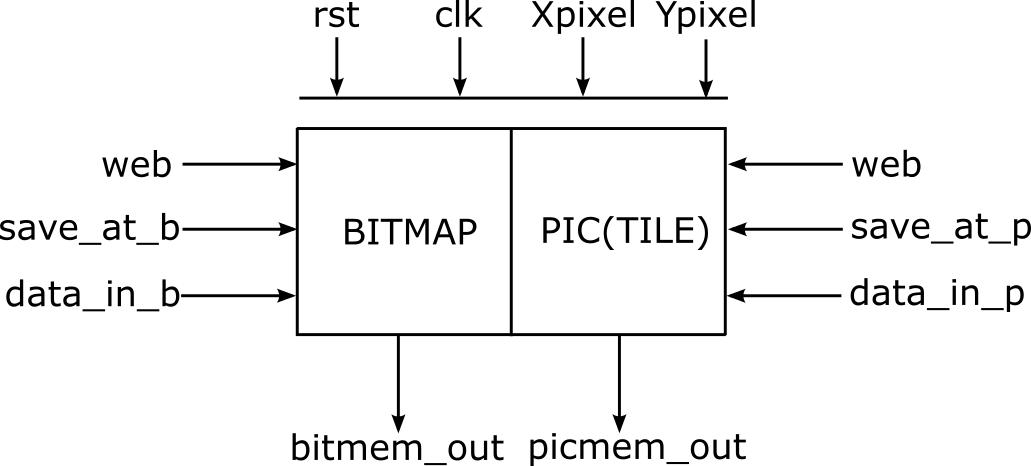
\includegraphics[width=1\textwidth]{drawings/pic_mem.png}}
	\caption{Blockschema över bildminnet}
\end{figure}

Bildminnet är uppdelat i två kolumner, där ena hälften använder tiles och andra hälften använder en bitmap. Bitmapminnet innehåller 320x480 bitars blockram för en svartvit representation av alla pixlar på vänstra skärmhalvan. Bildminnet för tiles innehåller 40x30 rader.

Varje del har en write\_enable-signal, en save\_at-signal och en data\_in-signal. När write\_enable ettställs ersätts innehållet på adressen save\_at med data\_in. Bitmapminnet använder endast sista biten i data\_in\_b, medans hela data\_in\_p används.

Xpixel och Ypixel används för att bestämma om picmem\_out eller bitmem\_out ska uppdateras, för att undvika overflow i minnena.

\subsection{VGA-motor}
\begin{figure}[h!]
	\makebox[\textwidth][c]{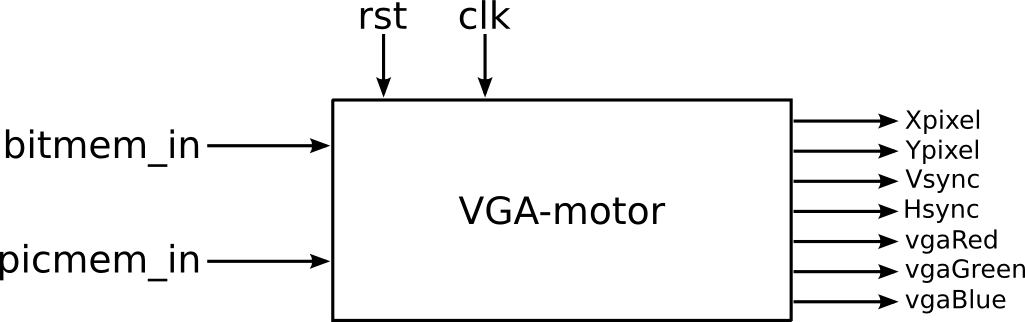
\includegraphics[width=1\textwidth]{drawings/vga_motor.png}}
	\caption{Översiktligt blockschema över VGA-motorn}
\end{figure}

\section{Mjukvara}
\subsection{Hjälpmedel}

\subsection{Calc}

\subsection{Beräkningar}
\subsubsection{Reverse polish}
\subsubsection{Eval\_fn}
\subsubsection{Division}

\subsection{Grafer}
\subsubsection{Axlar}
\subsubsection{Utritning}

\subsection{IO}
\subsubsection{Print-num}
\subsubsection{TODO}

\section{Slutsatser}
\section{Referenser}
\section{VHDL-dokumentation}
\subsection{CPU}

\subsection{Tangentbordsmotor}

\subsection{Bildminne}

\subsection{VGAMotor}

\subsection{Testbenches}
Inte själva VHDL-koden utan en förklaring av den. Typiskt en förklaring av varje process.


\end{document}          
